%!TEX root=../oi-magistr-si.tex
\section[AOS - SOA]{Co je to architektura zaměřená na služby (SOA)? Základní pojmy, vztah k objektově orientované architektuře. Konceptuální model a formalismy pro modelování SOA.}

\subsection{Architektura zaměřená na služby (SOA)}
SOA je model softwarové architektury, kde byznys funkcionalita je logicky oddělena (grupována).

\begin{itemize}[itemsep=0px]
\item \textbf{sada návrhových principů} používaných během vývoje systému a integrace.
\item SOA je styl návrhu takových aplikací, které jsou složeny z vícero odlišných částí (poskytující funkcionalitu jako služby jiným aplikacím), které mají definované jednoduché rozhraní.
\item SOA nabízí množinu služeb, které mohou být použity v různých business doménách
\item způsob, jak spolu mohou dvě \textbf{distribuované aplikace} komunikovat, i když běží na různých \textbf{platformách} a \textbf{technologiích}
\item definuje \textbf{rozhraní} ve smyslu protokolů (WSDL, XML, HTTP, UDDI, SOAP) a funkcionalit
\item dodržuje zásady loose coupling jak mezi jednotlivými službami, tak mezi službou a vrstvou, která leží pod ní
\item odděluje funkčnost do nezávislých menších jednotek (nebo services), které jsou dostupné na síti
\end{itemize}

\textit{\uv{SOA is a style of architecting applications in such a way that they are composed of discrete software agents that have simple, well defined interfaces and are orchestrated through a loose coupling to perform a required function.}}

\subsubsection{Webová služba}
Služby zahrnují neasociované, \textit{loosely coupled} jednotky funkcionality, kter0 jsou přístupn0 přes internet dalším programům. Služby (a jejich konzumeři) komunikují mezi sebou předáváním dat ve \textit{well-defined} sdíleném formátu (např. XML, JSON).

\begin{itemize}[itemsep=0px]
\item \textbf{loose coupling} - services udržují vztah, který minimalizuje závislosti a udržuje jen minimální povědomí o ostatních službách.
\item \textbf{abstrakce} - služby skrývají logiku s vnějškem (my se jen dotážeme, a dostaneme naše data)
\item \textbf{znovupoužitelnost} - logika je rozdělena do dalších služeb za účelem dalšiho znovupoužití
\item \textbf{kompozice} - více služeb může spolupracovat (kompozice) a tvořit tak plnohodnotnou aplikaci (\textit{mashup})
\end{itemize}


\subsubsection*{Stateless vs. Stateful service}
\paragraph{Stateful:}
\begin{itemize}[itemsep=0px]
\item každý dotaz musí obsahovat veškerá data (kontext, stav) - stavová služba si \textbf{drží session} mezi klientem a serverem.
\item \textbf{hůře se škáluje} (pokud máme hodně klientů musíme si někde držet kontext pro každého klienta zvlášť).
\end{itemize}
\paragraph{Stateless:}
\begin{itemize}[itemsep=0px]
\item bezestavový znamená, že server si \textbf{nedrží} žádnou \textbf{session}
\item každý \textbf{request} je iz\textbf{}olovaná transakce (request musí obsahovat všechny potřebná data) a nemá vztah k žádnému předchozímu requestu
\item \textbf{lépe škálovatelné} (není nutnost držet kontext pro každého klienta)
\item lépší zotavení z chyb (díky izolovaným requestům)
\item \textbf{spolehlivost}
\end{itemize}

\subsubsection*{Idempotentní requesty}
Služba by měla zajišťovat omezení na idempotentní requesty. To znamená, že \textbf{duplicitní požadavky} mají \textbf{stejný efekt} jako unikátní požadavek.Toto omezení umožní poskytovateli a klientovi zlepšit celkovou spolehlivost služby
pouze tím, že se v případě výskytu chyby požadavek zopakuje.

Metody PUT a DELETE v HTTP protokolu jsou definovány jako idempotentní. Metody GET, HEAD, OPTIONS a TRACE, jsou předepsány jako bezpečné, a měly by být rovněž idempotentní. Oproti tomu POST metoda nemusí být nutně idempotentní, a proto se zasláním shodného POST požadavku vícekrát, může navíc ovlivňovat stav nebo způsobit další nežádoucí účinky.

\paragraph{Vztah k objektově orientované architektuře}
\begin{itemize}[itemsep=0px]
\item používání komponent
\item dodržování zásad \textit{low coupling} a \textit{high cohesion}
\item komunikace přes rozhraní
\item abstrakce
\end{itemize}

\subsection{Konceptuální model}
Koncept SOA je založen na interakci mezi dvěma klíčovými entitami: poskytovatelem a spotřebitelem služeb. Každá služba je specifikovaná svým popisem, na základě kterého spotřebitel vyhledá odpovídající službu v registru služeb a naváže s ní komunikaci.

\begin{figure}[h!]
\centering
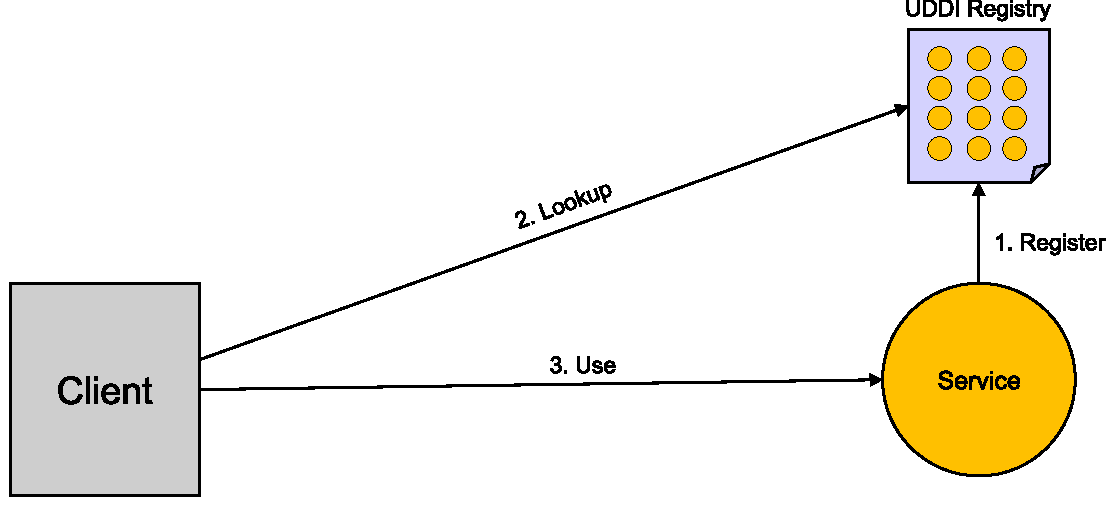
\includegraphics[width=100mm]{09/images/uddi-concept}
\end{figure}
